\documentclass[handout]{beamer}
\usetheme{Madrid}
\usecolortheme{default}

% \geometry{paperwidth=11in, paperheight=8.5in}

\usepackage[backend=biber]{biblatex}
\bibliography{cite.bib}


\usepackage{pgfpages}
\pgfpagesuselayout{resize to}[letterpaper, landscape, border shrink=0.5in]
\setbeamertemplate{footline}{} % Removes the footer
\usepackage{url, mathrsfs}
\usepackage{amsmath, amssymb, amsthm}
\usepackage{graphicx}
\usepackage{tikz}
\usetikzlibrary{positioning, calc, decorations.pathmorphing, shapes.gates.logic.US, arrows.meta}
\usepackage{quiver}
\usepackage{bm}
\usepackage{bbm}

% TikZ libraries
\usetikzlibrary{cd}

% Macros from the paper
\newcommand{\F}{\mathbb{F}}
\newcommand{\Rring}{R}
\newcommand{\Z}{\mathbb{Z}}
\newcommand{\N}{\mathbb{N}}

\title{Cyclic Error Correcting Codes}
\author{Grant Yang}
\institute{MATH 380 Spring 2026}
\date{June 2026}

\begin{document}

\begin{frame}[noframenumbering]
    \titlepage
\end{frame}

\begin{frame}{Introduction}
    \begin{itemize}
        \item  We would like to be able to communicate over noisy channels and correct any errors that occur in transit. 
        \item Interested in \emph{block codes}, where we encode each $k$ bit block (our \emph{message}) into an $n$ bit long \emph{codeword}.
        \item Restrict ourselves to \emph{linear} and \emph{cyclic} codes because they have some really nice properties.
        \begin{itemize}
            \item Famous coding schemes including Reed-Solomon and Hamming codes are linear and cyclic.
        \end{itemize}
        \item Working over the finite field $\mathbb F_2$:
        \begin{table}[H]
        \centering
        \begin{tabular}{|c||c|c| c |c||c|c|}
             \cline{1-3} \cline{5-7}
             $\times$ & $\mathbf 0$ & $\mathbf 1$ & \hspace{1em} & $+$ & $\mathbf 0$ & $\mathbf 1$  \\
             \cline{1-3} \cline{5-7}
             $\mathbf 0$ & $0$ & $0$ & \hspace{1em} & $\mathbf 0$ & $0$ & $1$ \\
             \cline{1-3} \cline{5-7}
             $\mathbf 1$ & $0$ & $1$ & \hspace{1em} & $\mathbf 1$ & $1$ & $0$ \\
             \cline{1-3} \cline{5-7}
        \end{tabular}
        \label{multf2}
        \end{table}
        \item Messages can be viewed as vectors $(m_1,\dots, m_k) \in \mathbb F_2^k$ or as polynomials $m_1 x^{k-1} + \dots+m_k \in \mathbb F_2[x]$. Similarly for codewords $(c_1,\dots,c_n)\in \mathbb F_2^n\iff c_1 x^{n-1}+\dots + c_n \in \mathbb F_2[x]$.
    \end{itemize}
   
\end{frame}

\begin{frame}{The Quotient Ring $R = \F_2[x]/\langle x^n - 1\rangle$}
    \textbf{Homework 4, \S2.6 Exercise 13} \\
    Let $G$ be a Gr\"obner basis. For any $f,g \in \F_2[x]$:
    \begin{enumerate}
        \item $\overline{f}^G = \overline{g}^G \iff f-g \in \langle x^n-1\rangle$.
        \item $\overline{f+g}^G = \overline{f}^G + \overline{g}^G$.
        \item $\overline{\overline{f}^G\overline{g}^G}^G = \overline{fg}^G$.
    \end{enumerate}
    \vspace{0.3cm}
    $R$ is the set of remainders modulo $x^n-1$, and it is a ring:
    \begin{itemize}
        \item Addition and multiplication are defined modulo $G$.
        \item Shifting $abcd \mapsto bcda$ corresponds to multiplication by $x$:
        \[(c_1 x^{n-1} + \dots + c_n) \cdot x \equiv c_2 x^{n-1} + \dots + c_1 \pmod{x^n-1}. \]
        This is why we want to use polynomials!
    \end{itemize}
\end{frame}

\begin{frame}{Ideals and Cyclic Codes}

    \begin{theorem}
        There is a bijection between cyclic linear codes of length $n$ and ideals of $R = \F_2[x]/\langle x^n - 1\rangle$, and every ideal $I \subseteq R$ is principal, i.e. $I = \langle g(x)\rangle_R$ for some $g(x) \in R$.
    \end{theorem}

    \begin{itemize}
        \item Let $C \subseteq R$ be the set of valid codewords for any cyclic code.
        \item Linearity: For any $c, c' \in C$, we must have $c+c' \in C$.
        \item Cyclic: For any $c \in C$, we must have $x \cdot c \in C$.
        \begin{itemize}
            \item Multiplication by $x$ is a circular shift.
            \item This implies $h(x) \cdot c \in C$ for any $h(x) \in R$, so $C$ is an ideal.
        \end{itemize}
        \item We can consider the ideal $\langle C \rangle \subseteq \mathbb F_2[x]$, and apply the fact that every ideal in $\mathbb F_2[x]$ is principal along with properties of remainders.
        \begin{itemize}
            \item We can show the generator $g \in \mathbb F_2[x]$ of $\langle C \rangle \subseteq \mathbb F_2[x]$ satisfies $g \in R$ and also generates $C = \langle g\rangle_R$.
        \end{itemize}
    \end{itemize}
\end{frame}

\begin{frame}{Hamming Distance}
    \begin{itemize}
        \item Let $d_H : R \to \mathbb N$ be the \emph{Hamming distance} between two codewords, the number of bits at which they differ.
        \item Define the \emph{Hamming weight} of a codeword $c \in R$ to be $d_H(0, c)$.
        \item $d_H(c_1,c_2)=d_H(0,c_2-c_1)$, and recall that if $c_1,c_2 \in C$, then $c_2-c_1 \in C$, where $C$ is the set of \emph{valid} codewords.
        \item The minimum codeword separation is
            \[d = \min_{c_1,c_2 \in C} d_H(c_1,c_2) = \min_{c \in C} d_H(0,c).\]
        \item We can write the codeword received as the original codeword plus errors, remembering that addition is XOR: \[c'(x) = c(x) + e(x).\]
        \item Any errors with Hamming weight less than
        $\left\lfloor \frac{d-1}{2} \right\rfloor$
        are correctable.
        \begin{itemize}
            \item We stay close to the valid codeword we originated from, as we cannot pass over the halfway point to a different codeword.
        \end{itemize}
    \end{itemize}
\end{frame}

\begin{frame}{The Hamming Cube}
    \vspace{1em}
    \begin{figure}
        \centering
            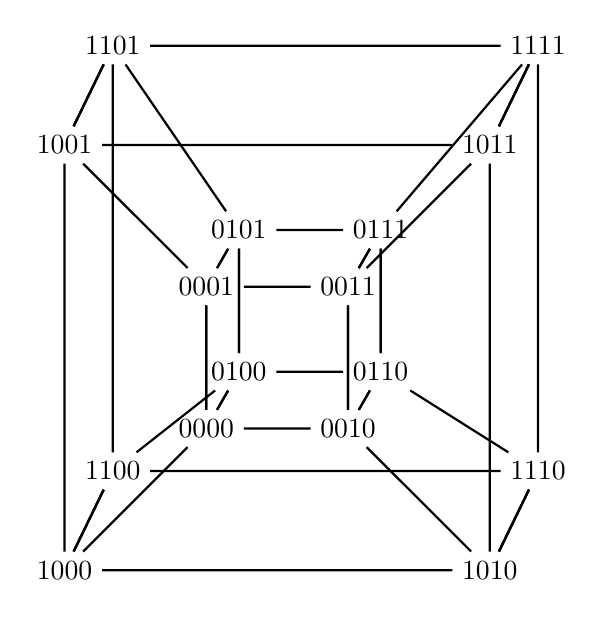
\begin{tikzpicture}[scale=1.8]
	 \tikzstyle{vertex}=[rectangle]
	 \tikzstyle{edge} = [draw,thick,-,black]
	 \node[vertex] (v0) at (0,0) {$0000$};
	 \node[vertex] (v1) at (0,1) {$0001$};
	 \node[vertex] (v2) at (1,0) { $0010$};
	 \node[vertex] (v3) at (1,1) { $0011$};
	 \node[vertex] (v4) at (0.23, 0.4) { $0100$};
	 \node[vertex] (v5) at (0.23,1.4) { $0101$};
	 \node[vertex] (v6) at (1.23,0.4) { $0110$};
	 \node[vertex] (v7) at (1.23,1.4) { $0111$};
	 \node[vertex] (v8) at (-1,-1) { $1000$};
	 \node[vertex] (v9) at (-1,2) { $1001$};
	 \node[vertex] (v13) at (-0.66,2.7) { $1101$};
	 \node[vertex] (v12) at (-0.66,-0.3) { $1100$};
	 \node[vertex] (v10) at (2,-1) { $1010$};
	 \node[vertex] (v14) at (2.34,-0.3) { $1110$};
	 \node[vertex] (v11) at (2,2) { $1011$};
	 \node[vertex] (v15) at (2.34,2.7) { $1111$};
	 \draw[edge] (v0) -- (v1) -- (v3) -- (v2) -- (v0);
	 \draw[edge] (v0) -- (v4) -- (v5) -- (v1) -- (v0);
	 \draw[edge] (v2) -- (v6) -- (v7) -- (v3) -- (v2);
	 \draw[edge] (v4) -- (v6) -- (v7) -- (v5) -- (v4);
	 \draw[edge] (v8) -- (v9) -- (v13) -- (v12) -- (v8);
	 \draw[edge] (v0) -- (v4) -- (v12) -- (v8) -- (v0);
	 \draw[edge] (v1) -- (v9) -- (v13) -- (v5) -- (v1);
	 \draw[edge] (v2) -- (v10) -- (v14) -- (v6) -- (v2);
	 \draw[edge] (v8) -- (v10) -- (v14) -- (v12) -- (v8);
	 \draw[edge] (v3) -- (v11) -- (v15) -- (v7) -- (v3);
	 \draw[edge] (v10) -- (v11) -- (v15) -- (v14) -- (v10);
	 \draw[edge] (v9) -- (v11) -- (v15) -- (v13) -- (v9);
 \end{tikzpicture}
        % \caption{4-dimensional Hamming Hypercube.}
    \end{figure}
\end{frame}

\begin{frame}{Syndrome Decoding and Hamming Distance}
    The \textbf{syndrome} is the remainder 
    \[r(x) = \overline{c'(x)}^H= \overline{c(x)+e(x)}^H= \overline{c(x)}^H+\overline{e(x)}^H=\overline{e(x)}^H.\]
    \begin{theorem}
        Errors $e(x)$ with Hamming weight $\le \left\lfloor \frac{d-1}{2} \right\rfloor$ have unique syndromes.
    \end{theorem}
    \begin{proof}
    \begin{itemize}
        \item Let $e_1 \neq e_2$ be errors with weight $\le \left\lfloor \frac{d-1}{2} \right\rfloor$.
        \item Assume for contradiction that $\overline{e_1}^H = \overline{e_2}^H$. Then $\overline{e_1 - e_2}^H = 0$.
        \item This means $e_1 - e_2$ is a valid nonzero codeword.
        \item However, $\text{weight}(e_1 - e_2) \le \text{weight}(e_1) + \text{weight}(e_2) \le d-1$.
        \item This contradicts the fact that the minimum weight of a nonzero codeword is $d$.
        \item Thus, every error with weight $\le \left\lfloor \frac{d-1}{2} \right\rfloor$ has a unique syndrome.
    \end{itemize}
    \end{proof}
\end{frame}

\begin{frame}[t]{$\mathbb F_2$ Vector Spaces vs. $\mathbb F_2[x]$-modules}
    \begin{figure}
        \centering
        \begin{tikzcd}[ampersand replacement=\&]
            \& {\text{Messages}} \& {\text{Codewords}} \& {\text{Syndromes}} \\
            0 \& {\mathbb F_2^k} \& {\mathbb F_2^n} \& {\mathbb F_2^{n-k}} \& 0 \\
            0 \& {\langle g \rangle_R} \& R \& {R/\langle g \rangle_R} \& 0
            \arrow[from=1-2, to=1-3]
            \arrow[from=1-3, to=1-4]
            \arrow[from=2-1, to=2-2]
            \arrow["G", from=2-2, to=2-3]
            \arrow["H", from=2-3, to=2-4]
            \arrow[from=2-4, to=2-5]
            \arrow[from=3-1, to=3-2]
            \arrow[hook, from=3-2, to=3-3]
            \arrow[two heads, from=3-3, to=3-4]
            \arrow[from=3-4, to=3-5]
        \end{tikzcd}
    \end{figure}
\end{frame}

\begin{frame}{Hamming(7,4): Characteristics}
    \begin{itemize}
        \item $n=7, k=4$. $R = \F_2[x]/\langle x^7-1\rangle$.
        \item Generator $g(x) = x^3+x^2+1$.
        \item Minimum codeword separation of $d=3$.
        \item Can correct up to $\left\lfloor \frac{d-1}{2}\right\rfloor=1$ bit flip.
    \end{itemize}
    
    \begin{table}[h]
        \centering
        \def\arraystretch{1.7}
        \begin{tabular}{r ||c|c|c|c|c|c|c|c}
             $e(x)$ & $0$ & $1$ & $x$ & $x^2$ & $x^3$ & $x^4$ & $x^5$ & $x^6$ \\
             \hline
             $\overline{e(x)}^H$ & $0$ & $1$ & $x$ & $x^2$ & $x^2+1$ & $x^2+x+1$ & $x+1$ & $x^2+x$ \\
    
        \end{tabular}
        \caption{Syndromes for $H=\{g(x)\}=\{x^3+x^2+1\}$.}
        \label{tab:placeholder}
    \end{table}
\end{frame}

\begin{frame}{Hamming(7,4): Worked Example}
    Working with Gr\"obner basis $H=\{g(x)\}=\{x^3+x^2+1\}$.
    \begin{itemize}
        \item \textbf{Message:} $1010 \implies m(x) = x^3+x$.
        \item \textbf{Encode:} $c(x) = m(x)g(x) = x^6+x^5+x^4+x \implies 1110010$.
        \item Receive $c'(x) = x^5+x^4+x \implies \underline{\textbf 0}110010$.
        \item \textbf{Decode:} Syndrome $\overline{c'(x)}^H = x^2+x$.
        \item Lookup table: $x^2+x \mapsto e(x) = x^6$.
        \item Recover original codeword $c(x) = c'(x) + x^6\implies 1110010$.
    \end{itemize}
\end{frame}

\begin{frame}{Hamming(7,4): Systematic Encoding}

    Systematic Encoding: $c(x) = x^{n-k}m(x) - \overline{x^{n-k}m(x)}^H$.
    \begin{itemize}
        \item \textbf{Message:} $1010 \implies m(x) = x^3+x$.
        \item $x^3m(x) = x^6+x^4$. Remainder modulo $g$ is $1$.
        \item \textbf{Encode:} $c(x) = x^6+x^4+1 \implies \underline{1010}001$
        \begin{itemize}
            \item 3 parity bits appended.
            \item The first $k$ bits of the codeword matches the message!
        \end{itemize}
        \item Receive $c'(x)=x^4+1 \implies \underline{\textbf 0}010001$.
        \item \textbf{Decode:} Syndrome $\overline{c'(x)}^H = x^2+x$.
        \item Lookup table: $x^2 + x \mapsto e(x)=x^6$.
        \item Recover $c(x)=c'(x)+x^6=\underline{1010}001$.
    \end{itemize}
\end{frame}

\tikzset{
    >=Stealth,
    font=\sffamily,
    xor/.style={circle, draw, thick, inner sep=0pt, minimum size=6mm},
    % Cleaned up IEEE D Flip-Flop symbol (chevron only, no textual pins)
    dff/.style={
        rectangle, draw, thick, minimum width=0.8cm, minimum height=0.8cm,
        path picture={
            % Clock chevron precisely at the bottom center edge
            \draw[thick] ([xshift=-1.2mm]path picture bounding box.south) -- ++(1.2mm, 1.2mm) -- ++(1.2mm, -1.2mm);
        }
    },
    block/.style={rectangle, draw, thick, align=center},
    line/.style={draw, thick, ->},
    wire/.style={draw, thick},
    dot/.style={circle, fill, inner sep=1.2pt}
}

% ==========================================
% ENCODER SLIDE
% ==========================================
\begin{frame}{Systematic Encoder \& Meggitt Decoder}
    \begin{center}
    \resizebox{0.95\textwidth}{!}{
    \begin{tikzpicture}
        % Inputs
        % \node[anchor=south] at (-1.2, -1.9) {($0$-padded)};
        \node[anchor=east] (msg_in) at (0, -2) {Message $m(x)$};
        \node[anchor=east] (gnd) at (2.5, -0.5) {0 (GND)};
        
        % Shift Register & XORs (Using clean 'dff' style)
        \node[xor] (e_x1) at (3.5, -0.5) {$\oplus$};
        \node[dff] (e_d1) at (5.0, -0.5) {$D_1$};
        \node[dff] (e_d2) at (6.5, -0.5) {$D_2$};
        \node[xor] (e_x3) at (8.0, -0.5) {$\oplus$};
        \node[dff] (e_d3) at (9.5, -0.5) {$D_3$};
        
        \node[xor] (e_xf) at (9.5, -2) {$\oplus$}; % Feedback XOR
        
        % MUX Box
        \node[block, minimum width=1.2cm, minimum height=2.4cm] (mux) at (12, -1.25) {};
        \node[font=\bfseries, rotate=90] at (12, -1.25) {MUX};
        \node[right, font=\scriptsize] at (mux.west |- 0,-0.5) {1};
        \node[right, font=\scriptsize] at (mux.west |- 0,-2) {0};
        
        % Connections - Upper LFSR path
        \draw[line] (gnd) -- (e_x1);
        \draw[line] (e_x1) -- (e_d1);
        \draw[line] (e_d1) -- (e_d2);
        \draw[line] (e_d2) -- (e_x3);
        \draw[line] (e_x3) -- (e_d3);
        
        % D3 Output Splits
        \node[dot] (e_d3_dot) at (10.5, -0.5) {};
        \draw[wire] (e_d3.east) -- (e_d3_dot);
        \draw[line] (e_d3_dot) -- (mux.west |- 0,-0.5);
        \draw[line] (e_d3_dot) |- (e_xf.east); 
        
        % Data In Splits
        \node[dot] (msg_dot) at (1.5, -2) {};
        \draw[wire] (msg_in) -- (msg_dot);
        \draw[line] (msg_dot) -- (e_xf.west);
        
        % Data routing under LFSR to MUX
        \draw[line] (msg_dot) -- (1.5, -3.2) -| (11.0, -2) -- (mux.west |- 0,-2);
        
        % Feedback Path
        \coordinate (fb_line) at (9.5, -2.8);
        \draw[wire] (e_xf.south) -- (fb_line);
        \draw[wire] (fb_line) -- (3.5, -2.8);
        \draw[line] (3.5, -2.8) -- (e_x1.south);
        \draw[line] (8.0, -2.8) -- (e_x3.south); 
        \node[dot] at (8.0, -2.8) {};
        
        % Encoder Output
        \node[right=1cm of mux] (enc_out) {Codeword $c(x)$};
        \draw[line] (mux.east) -- (enc_out);
    \end{tikzpicture}
    }
    \end{center}
    
    Mux selects raw message (\texttt{0}) for first $k=4$ clock cycles, then selects shift register output (\texttt{1}) for $n-k=3$ cycles (parity bits).
    
    \begin{center}
    \resizebox{0.95\textwidth}{!}{
    \begin{tikzpicture}
        % Input
        \node[anchor=east] (rx_in) at (0, -6) {Received $c'(x)$};
        
        % Syndrome Register
        \node[xor] (d_x0) at (2.0, -6) {$\oplus$};
        \node[xor] (d_x1) at (3.5, -6) {$\oplus$};
        \node[dff] (d_d1) at (5.0, -6) {$D_1$};
        \node[dff] (d_d2) at (6.5, -6) {$D_2$};
        \node[xor] (d_x3) at (8.0, -6) {$\oplus$};
        \node[dff] (d_d3) at (9.5, -6) {$D_3$};
        
        % Pattern Matcher connection dots
        \node[dot] (pm_in1) at (5.75, -6) {};
        \node[dot] (pm_in2) at (7.25, -6) {};
        \node[dot] (pm_in3) at (10.25, -6) {};
        
        \draw[line] (d_x0) -- (d_x1);
        \draw[line] (d_x1) -- (d_d1);
        \draw[wire] (d_d1) -- (pm_in1); \draw[line] (pm_in1) -- (d_d2);
        \draw[wire] (d_d2) -- (pm_in2); \draw[line] (pm_in2) -- (d_x3);
        \draw[line] (d_x3) -- (d_d3);
        
        % Syndrome Register Feedback
        \node[dot] (d_d3_dot) at (11, -6) {};
        \draw[wire] (d_d3.east) -- (pm_in3);
        \draw[wire] (pm_in3) -- (d_d3_dot);
        \draw[wire] (d_d3_dot) -- (11, -5) -- (3.5, -5);
        \draw[line] (3.5, -5) -- (d_x1.north);
        \draw[line] (8.0, -5) -- (d_x3.north); 
        \node[dot] at (8.0, -5) {};
        
        % Pattern Detector
        \node[block, minimum width=5.0cm, fill=gray!10, rounded corners=2pt] (pm) at (8, -7.5) {Pattern Detector \\ (Match Syndrome: 110)};
        \draw[line] (pm_in1) -- (pm_in1 |- pm.north);
        \draw[line] (pm_in2) -- (pm_in2 |- pm.north);
        \draw[line] (pm_in3) -- (pm_in3 |- pm.north);
        
        % Delay Line
        \node[dot] (rx_dot) at (1.0, -6) {};
        \draw[wire] (rx_in) -- (rx_dot);
        \draw[line] (rx_dot) -- (d_x0.west);
        
        \draw[line] (rx_dot) -- (1.0, -9) -- (2.0, -9);
        
        % Increased multiplier to 1.3 to add generous breathing room between boxes
        \foreach \i in {1,...,7} {
            \node[dff] (dd\i) at (1.2 + \i*1.3, -9) {$D$};
            \ifnum\i>1
                \pgfmathtruncatemacro{\prev}{\i-1}
                \draw[line] (dd\prev) -- (dd\i);
            \fi
        }
        
        % Output Correction XOR
        \node[xor] (corr_x) at (11.5, -9) {$\oplus$};
        \draw[line] (dd7) -- (corr_x.west);
        
        \node[right=1cm of corr_x] (dec_out) {Corrected $c(x)$};
        \draw[line] (corr_x.east) -- (dec_out);
        
        % Pattern Detector Output & Correction Feedback
        \node[dot] (pm_dot) at (11.5, -7.5) {};
        \draw[wire] (pm.east) -- (pm_dot);
        \draw[line] (pm_dot) -- (corr_x.north); % Corrects the bit
        
        % Feedback to clear the syndrome state simultaneously
        \draw[wire] (pm_dot) -- (11.5, -8.25) -- (2.0, -8.25);
        \draw[line] (2.0, -8.25) -- (d_x0.south);
        \node[dot] at (11.5, -8.25) {};
    \end{tikzpicture}
    }
    \end{center}

    Linear Feedback Shift Register (LFSR) implements multiplication by $x$ in the ring $\mathbb F_2[x]/\langle x^3+x^2+1\rangle$.
\end{frame}

\begin{frame}
    \frametitle{References}
    \nocite{*}
    \printbibliography
\end{frame}

\end{document}
